\newcommand{\modelreality}{Modelering af Virkeligheden}
\newcommand{\topicone}{Aalborg PBL}
\newcommand{\topictwo}{Representation}
\newcommand{\topicthree}{Design}
\section*{\modelreality}

\begin{frame}{\modelreality}
\begin{itemize}
	\item \topicone
	\item \topictwo
\end{itemize}
\end{frame}
\begin{frame}{\modelreality}{\topicone} 
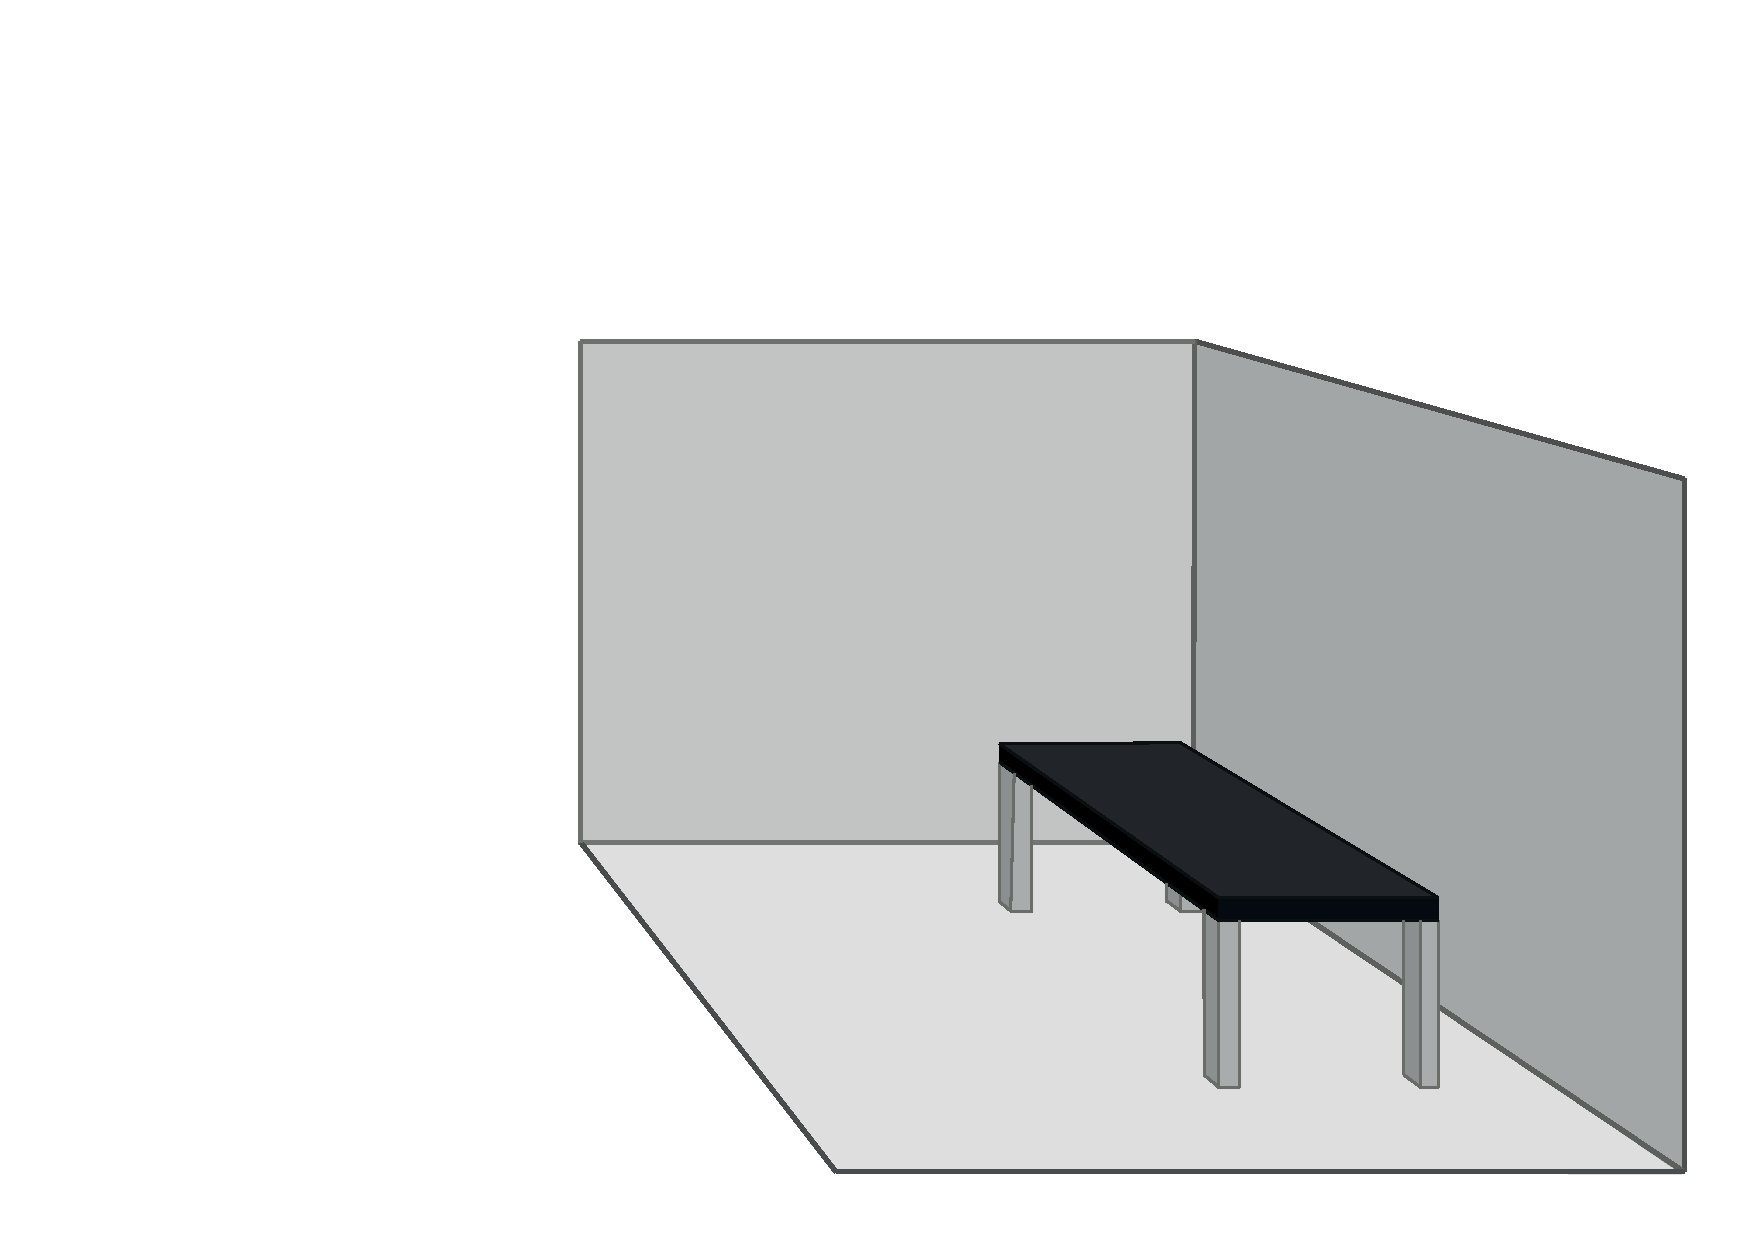
\includegraphics[width=\columnwidth]{input/rasmus/Rasmus1.pdf}
\end{frame}
\begin{frame}{\modelreality}{\topicone} 
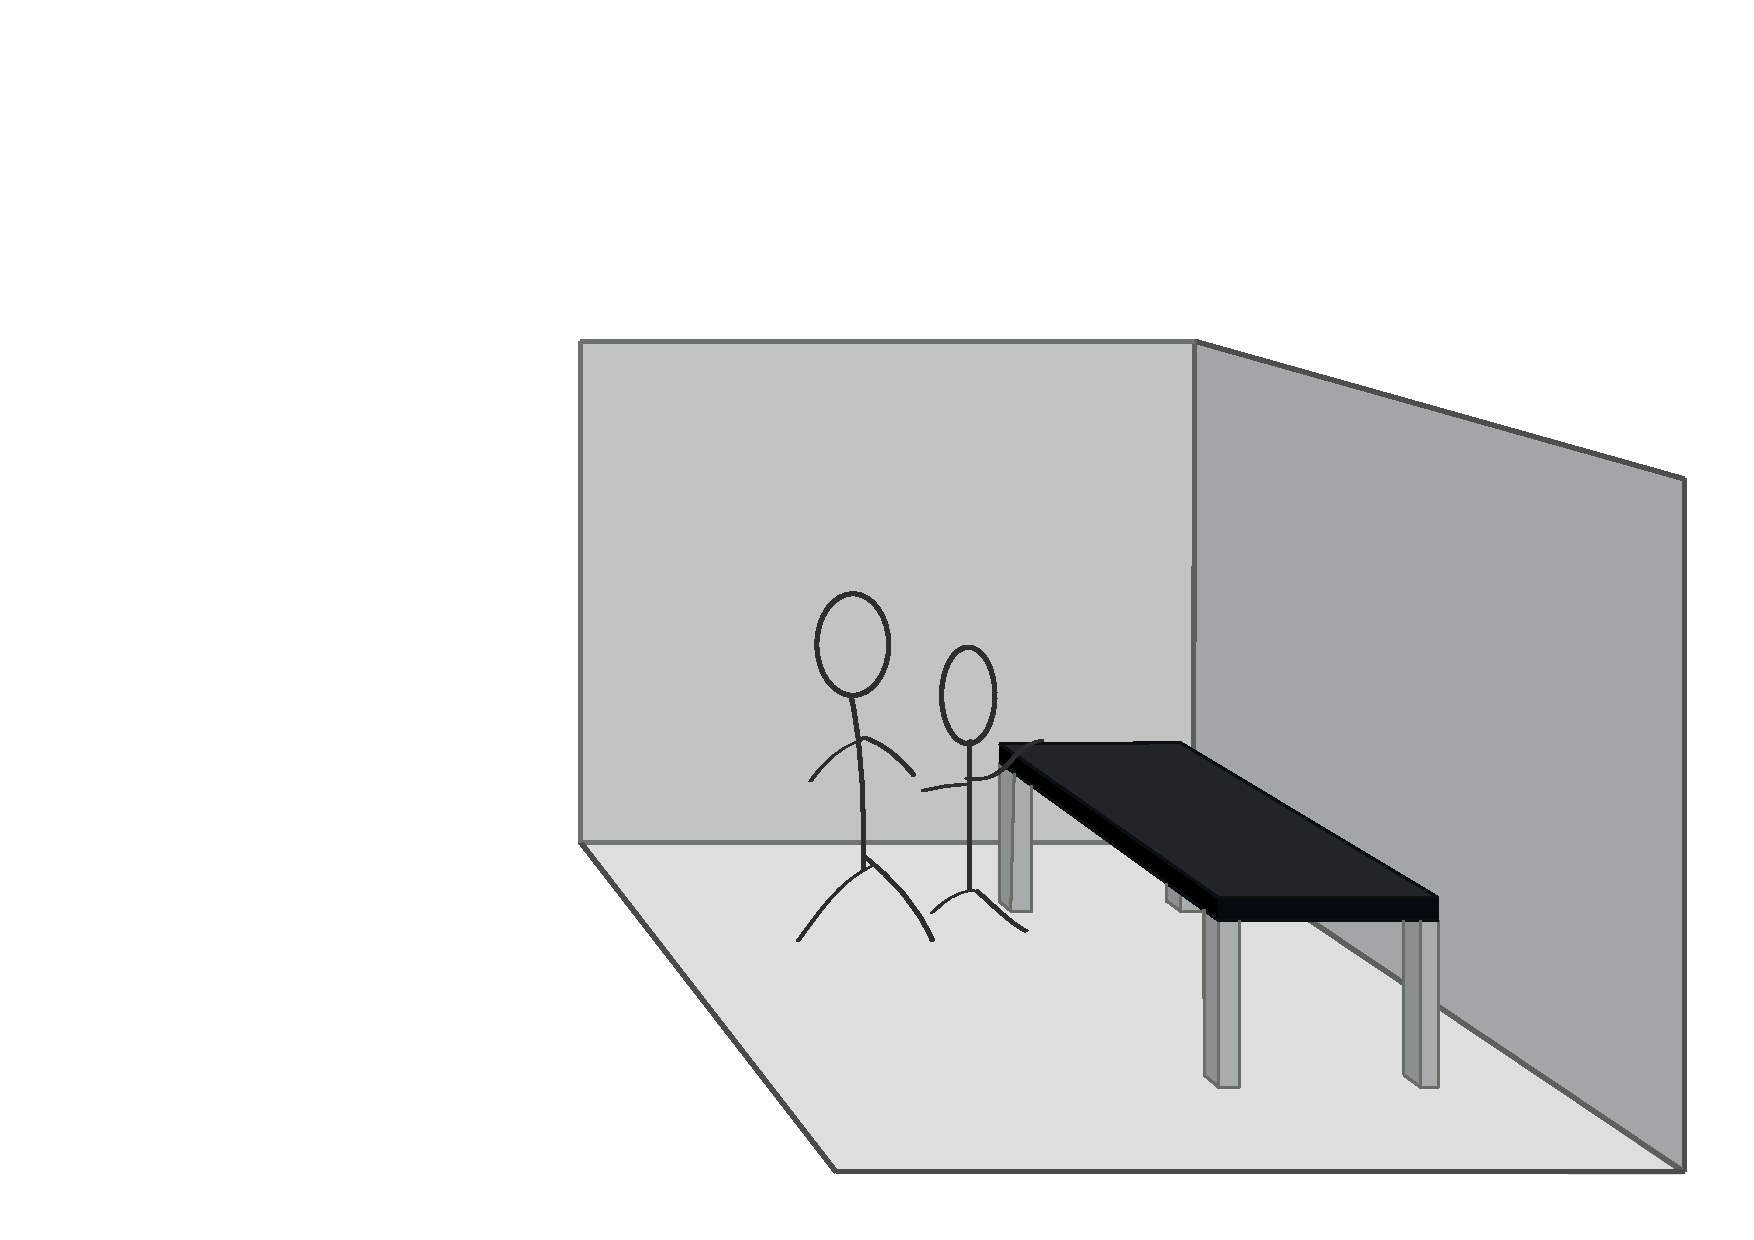
\includegraphics[width=\columnwidth]{input/rasmus/Rasmus2.pdf}
\end{frame}
\begin{frame}{\modelreality}{\topicone} 
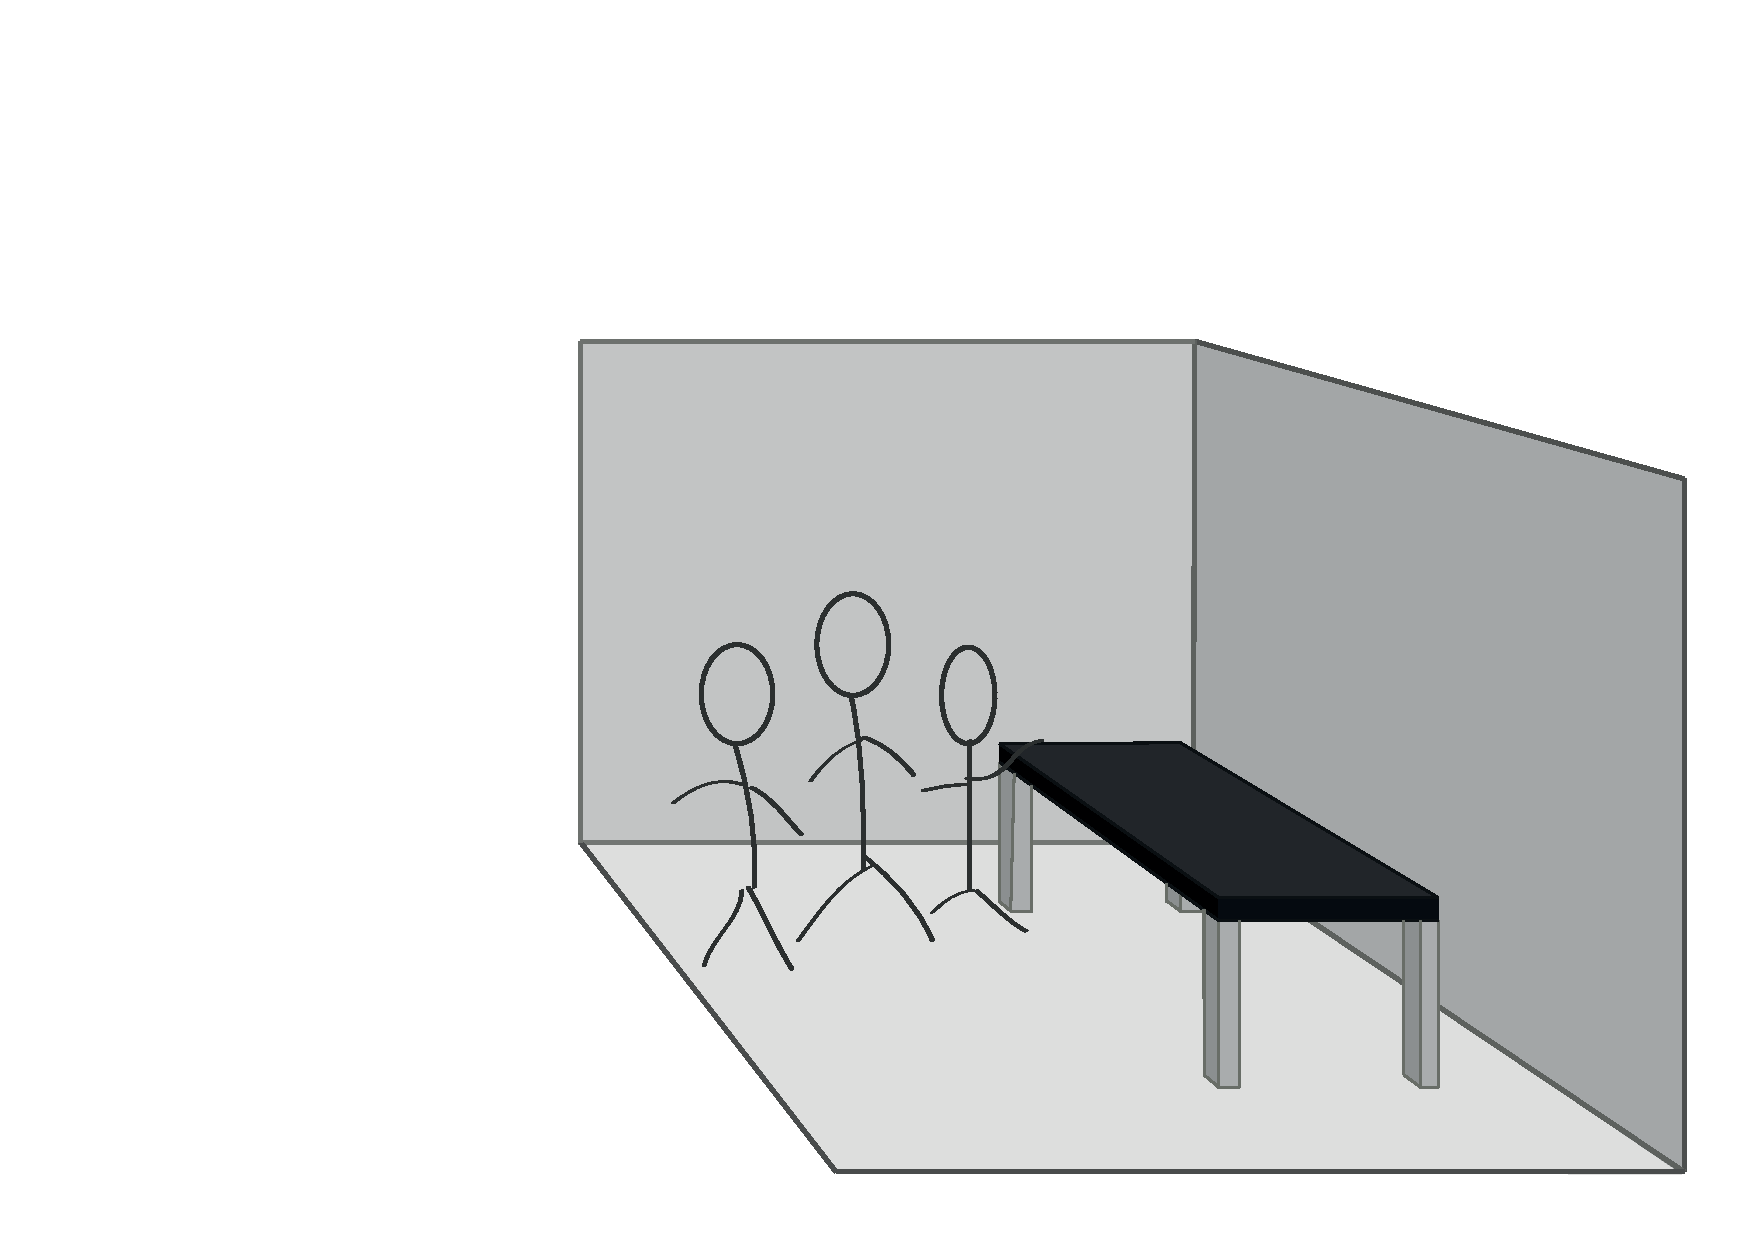
\includegraphics[width=\columnwidth]{input/rasmus/Rasmus3.pdf}
\end{frame}
\begin{frame}{\modelreality}{\topicone} 
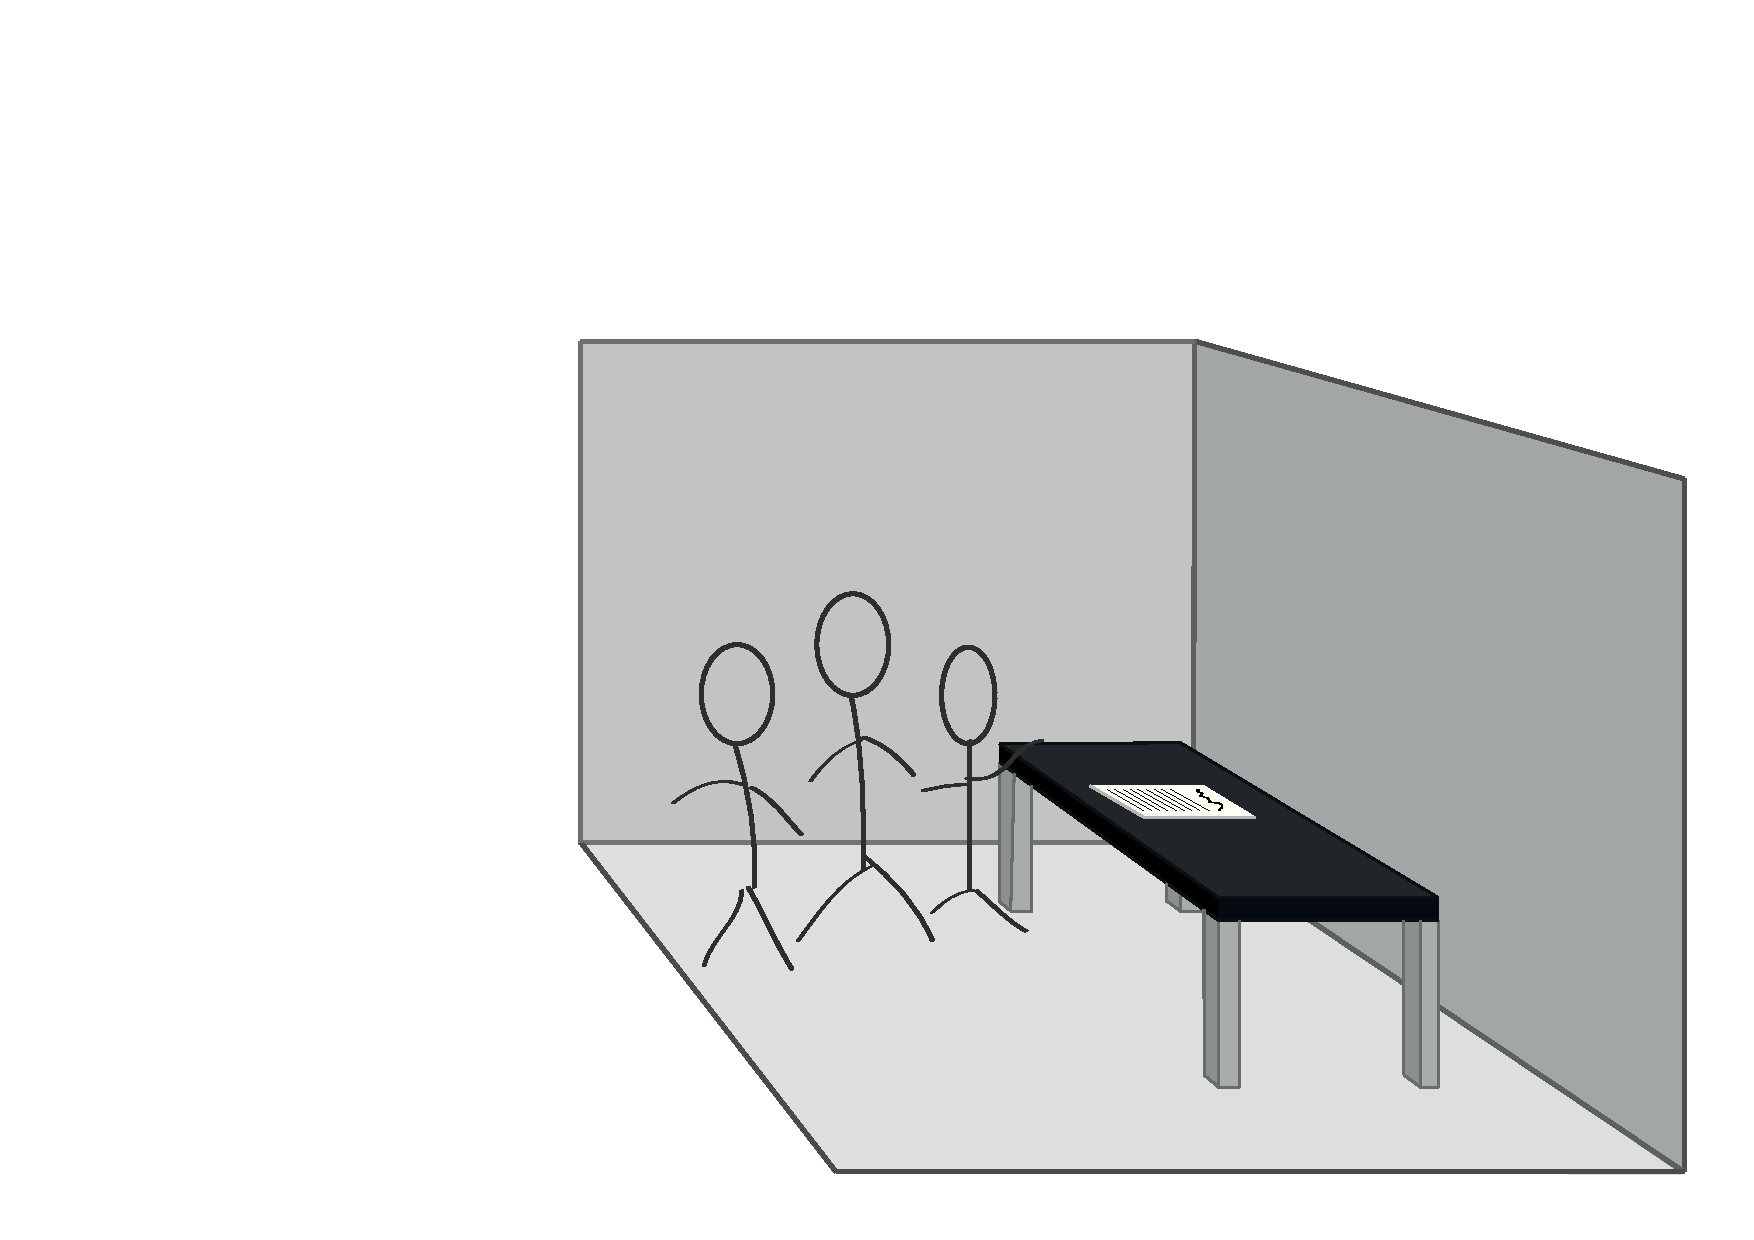
\includegraphics[width=\columnwidth]{input/rasmus/Rasmus4.pdf}
\end{frame}
\begin{frame}{\modelreality}{\topicone} 
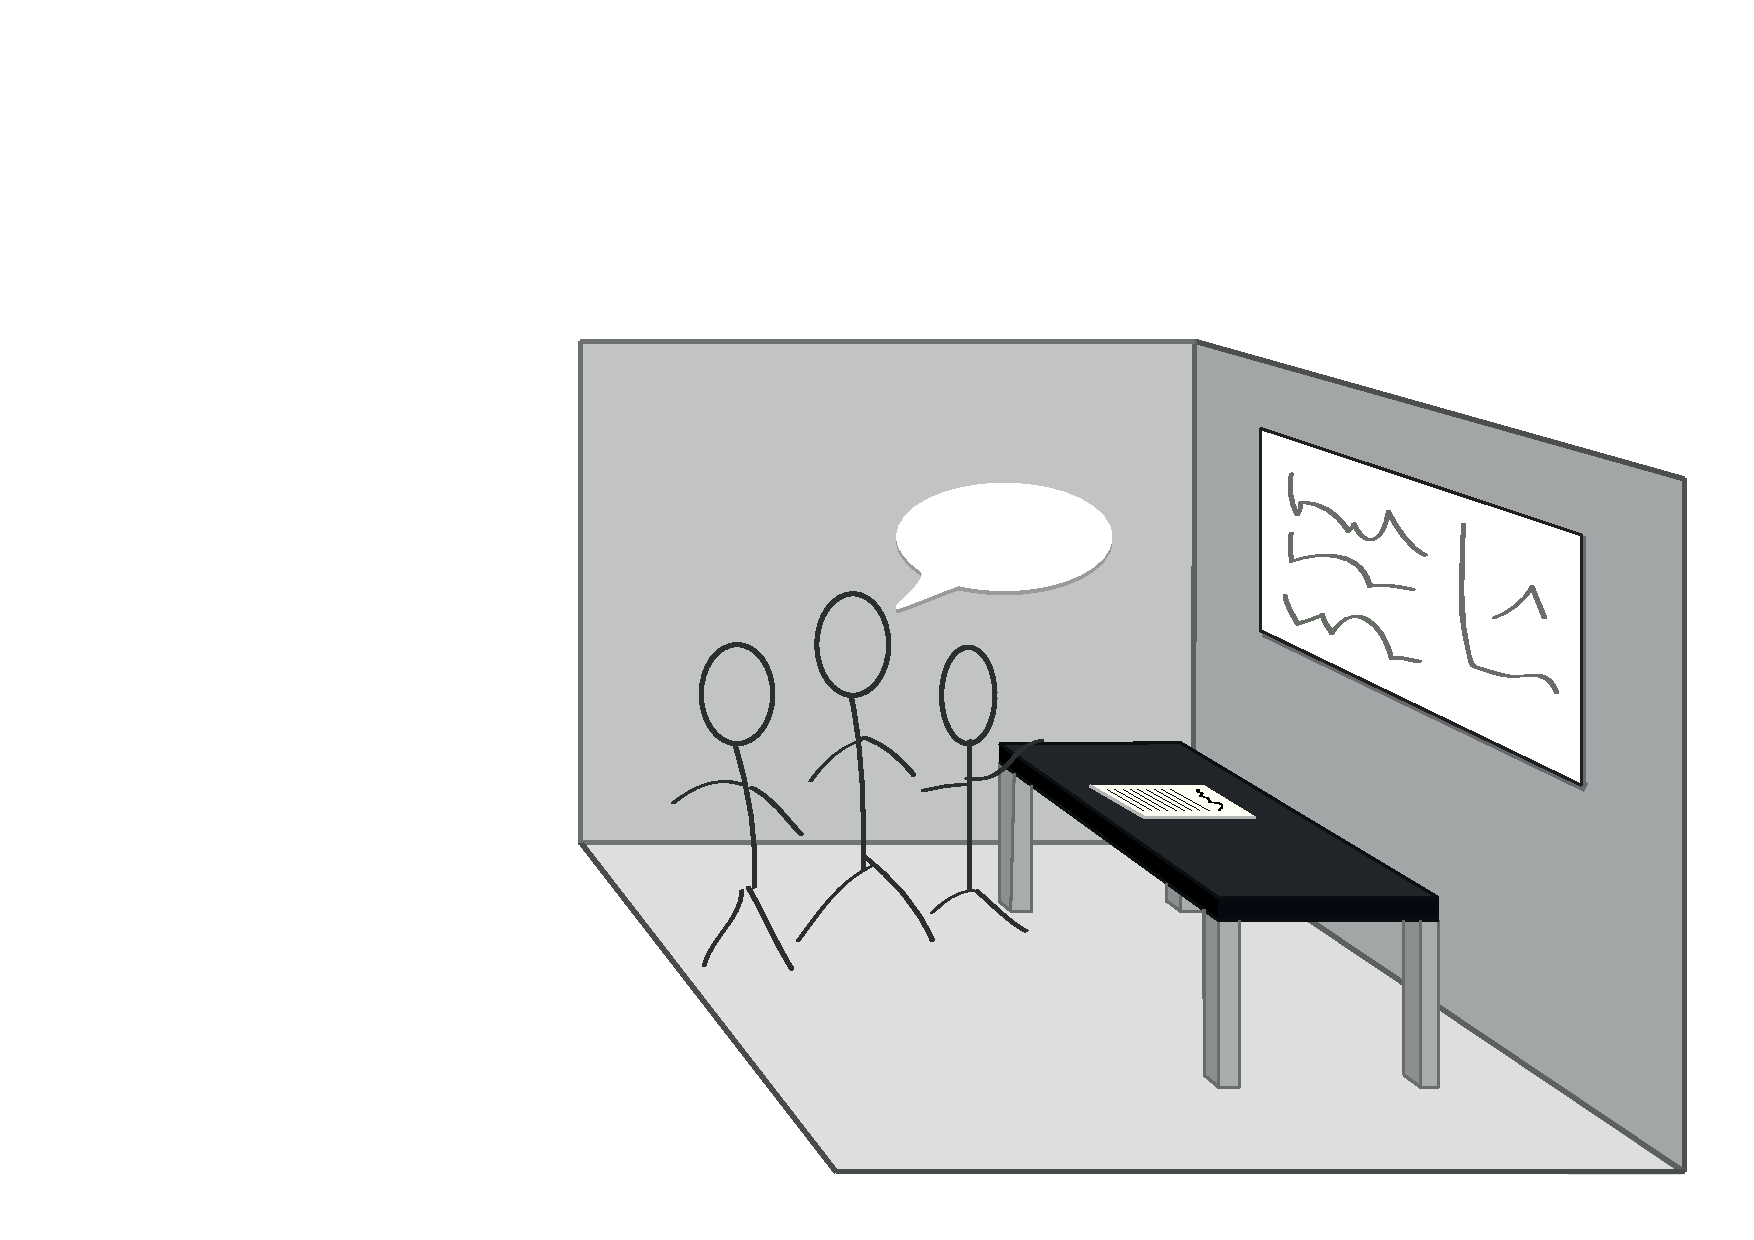
\includegraphics[width=\columnwidth]{input/rasmus/Rasmus5.pdf}
\end{frame}


\def\freqlist{1,2,3,4,5,6,6a,7,8,9}

\foreach \freq in \freqlist 
{
\begin{frame}{\modelreality}{\topictwo} 
\begin{figure}
\includegraphics[width=\columnwidth]{input/rasmus/two\freq.pdf}
\end{figure}
\end{frame}

} 

\begin{frame}{\modelreality}{\topicthree} 
\begin{figure}
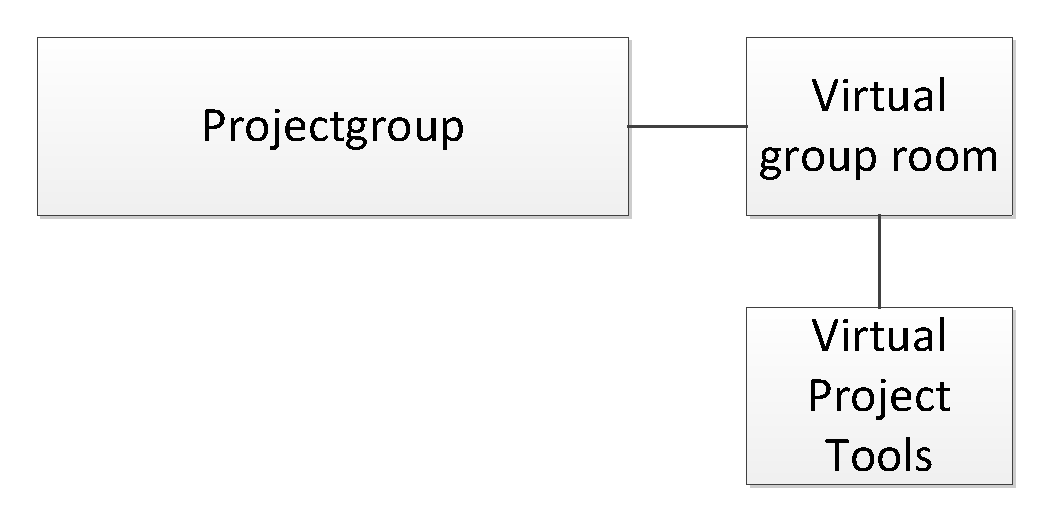
\includegraphics[width=\columnwidth]{input/rasmus/two10.pdf}
\end{figure}
\end{frame}

\begin{frame}{\modelreality}{\topicthree} 
\begin{figure}
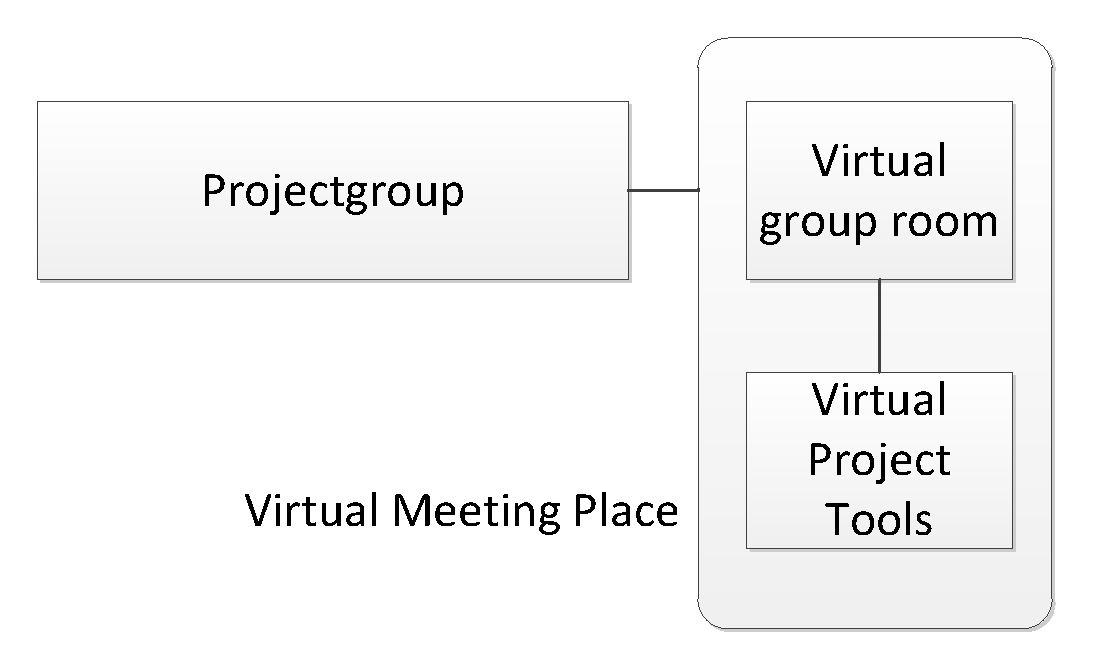
\includegraphics[width=\columnwidth]{input/rasmus/two11.pdf}
\end{figure}
\end{frame}